\documentclass[sigconf]{acmart}
\usepackage{algorithm}
\usepackage[export]{adjustbox}
\usepackage[noend]{algpseudocode}
\usepackage{todonotes}
\usepackage{xspace}
\usepackage{listings}
%
\usepackage{paralist}
\usepackage[compact]{titlesec}
\usepackage{balance}

\usepackage{xspace}
\usepackage{filecontents}
\usepackage[switch]{lineno}
\renewcommand{\linenumberfont}{\normalfont\tiny\color{red}}
\usepackage[dvipsnames]{xcolor}
\usepackage[most]{tcolorbox}

\newcommand{\mpifunc}[1]{\lstinline"MPI_#1"\xspace}
\newcommand{\prrte}[0]{\textsc{PRRTE}\xspace}
\newcommand{\pmix}[0]{\textsc{PMIx}\xspace}
\newcommand{\orte}[0]{\textsc{Open~RTE}\xspace}
\newcommand{\ompi}[0]{\textsc{Open~MPI}\xspace}
\newcommand{\mpi}[0]{\textsc{MPI}\xspace}
\newcommand{\arm}[0]{Arm\xspace}
\newcommand{\oshmem}[0]{\textsc{OpenSHMEM}\xspace}
\newcommand{\sve}[0]{\textsc{SVE}\xspace}
\newcommand{\armie}[0]{\textsc{ArmIE}\xspace}
\newcommand{\ddt}[0]{\textsc{DDT}\xspace}
\newcommand{\acle}[0]{\textsc{ACLE}\xspace}

\newcommand{\imb}[0]{\textsc{IMB}\xspace}

\def\BibTeX{{\rm B\kern-.05em{\sc i\kern-.025em b}\kern-.08emT\kern-.1667em\lower.7ex\hbox{E}\kern-.125emX}}

\copyrightyear{2019}
\acmYear{2019}
\acmConference[EuroMPI 2019]{26th European MPI Users' Group Meeting}{September 11--13, 2019}{Zürich, Switzerland}
\acmBooktitle{26th European MPI Users' Group Meeting (EuroMPI 2019), September 11--13, 2019, Zürich, Switzerland}
\acmPrice{15.00}
\acmDOI{10.1145/3343211.3343225}
\acmISBN{978-1-4503-7175-9/19/09}

\begin{document}

\title{Using Advanced Vector Extensions AVX-512 for MPI Reduction}

\author{Dong Zhong}
\email{dzhong@vols.utk.edu}
%\orcid{0000-0002-7651-2059}
\affiliation{%
  \institution{The University of Tennessee}
  \streetaddress{1122 Volunteer Blvd}
  \city{Knoxville}
  \state{TN}
  \postcode{37996}
  \country{USA}
}

\author{Qinglei Cao}
\email{qcao3@vols.utk.edu}
\affiliation{%
  \institution{The University of Tennessee}
  \streetaddress{1122 Volunteer Blvd}
  \city{Knoxville}
  \state{TN}
  \postcode{37996}
  \country{USA}
}

\author{George Bosilca}
\email{bosilca@icl.utk.edu}
\orcid{0000-0003-2411-8495}
%
\affiliation{%
  \institution{The University of Tennessee}
  \streetaddress{1122 Volunteer Blvd}
  \city{Knoxville}
  \state{TN}
  \postcode{37996}
  \country{USA}
}

\begin{abstract}
  As the scale of high-performance computing (HPC) systems continues to grow,
  researchers are devoted themselves to implore increasing levels of parallelism
  to achieve optimal performance.
  %
  Recently, the processors support wide vector extensions,
  vectorization becomes much more important to exploit the potential peak performance of
  target architecture.
  %
  Novel processor architectures, such as, Intel AVX-512 architecture introduced 512-bit extensions
  to the 256-bit Advanced Vector Extensions (SIMD) instructions for x86 instruction set architecture (ISA).
  The new architecture emploied new capabilities such as masked execution, vector mathematical functions, as well as a small set of new instructions for mathematical library support. These new features allow for better compliance with long vector load, store and also reduction operations.
  %
  ARM's new Armv8-A
  architecture, introduce \emph{Scalable Vector Extension} (\sve)
  - an optional separate architectural extension with a new set of A64
  instruction encodings, which enables even greater parallelisms.

  In this paper, we propose new optimized strategies by utilizing AVX-512 instructions to provide
  vector based reduction improving time to solution performance of MPI reduction operations.
%
  With these optimizations, we not only provide a higher-parallelism for a single node,
  but also achieve a more efficient communication scheme of message exchanging.
  The resulting efforts have been implemented in the context of \ompi, providing
  efficient and scalable capabilities of AVX-512 usage and extending the possible
  implementatios of AVX-512 to a larger range of programming and execution paradigms.
%
  The evaluation of the resulting software stack under different scenarios tested with
  Skylake processor demonstrates that the solution is at the same time generic and efficient.

\end{abstract}

%
\begin{CCSXML}
<ccs2012>
<concept>
<concept_id>10010520.10010521.10010537</concept_id>
<concept_desc>Computer systems organization~Distributed architectures</concept_desc>
<concept_significance>500</concept_significance>
</concept>
<concept>
<concept_id>10010520.10010521.10010542.10010546</concept_id>
<concept_desc>Computer systems organization~Heterogeneous (hybrid) systems</concept_desc>
<concept_significance>300</concept_significance>
</concept>
<concept>
<concept_id>10010520.10010575.10010577</concept_id>
<concept_desc>Computer systems organization~Reliability</concept_desc>
<concept_significance>300</concept_significance>
</concept>
<concept>
<concept_id>10010520.10010575.10011743</concept_id>
<concept_desc>Computer systems organization~Fault-tolerant network topologies</concept_desc>
<concept_significance>300</concept_significance>
</concept>
<concept>
<concept_id>10011007.10010940.10011003.10011005</concept_id>
<concept_desc>Software and its engineering~Software fault tolerance</concept_desc>
<concept_significance>300</concept_significance>
</concept>
<concept>
<concept_id>10011007.10011006.10011041.10011048</concept_id>
<concept_desc>Software and its engineering~Runtime environments</concept_desc>
<concept_significance>300</concept_significance>
</concept>
</ccs2012>
\end{CCSXML}

\ccsdesc[500]{Computer systems organization~Distributed architectures}
\ccsdesc[300]{Computer systems organization~Heterogeneous (hybrid) systems}
\ccsdesc[300]{Computer systems organization~Reliability}
\ccsdesc[300]{Computer systems organization~Fault-tolerant network topologies}
\ccsdesc[300]{Software and its engineering~Software fault tolerance}
\ccsdesc[300]{Software and its engineering~Runtime environments}

\keywords{OpenMPI, Intel AVX, AVX-512, Single instruction multiple data,
Long vector operation, Local reduction, MPI operation
}

%
\maketitle

\section{Introduction}\label{sec:intro}
The need to satisfy the scientific computing community's increasing
computational demands leads to larger HPC systems with more complex architectures,
which provides more opportunities to enrich multiple levels of parallelism.
%
Lots of researchers are focuing on exploiting data level parallelism by vector
execution and code vectorization~\cite{Vectorizing-Compilers} which leads HPC
systems to equip with vector processors.
%
Comparing to traditioanal scalar processors, extension vector processors support
Single Instruction Multiple Data (SIMD) and more powerful instructions operate
on vectors with multiples elements involved rather than single element which
could achieve maximum computational power.
%

There are efforts to keep improving the vector processors by increasing the vector
length and adding new vector instructions.
Intel starts from most vector integer SSE and AVX instructions, then expand to
Haswell instructions as 256 bits (AVX2),
the more advanced processor Knights Landing~\cite{avx-info} introduced
AVX-512~\cite{Intelref} support 512-bit wide SIMD registers (ZMM0-ZMM31)
as in Fig\ref{fig:avx_mms}. The lower 256-bits of the ZMM registers are
aliased to the respective 256-bit YMM registers and the lower 128-bit are
aliased to the respective 128-bit XMM registers;
%

These instructions represent a significant leap to 512-bit SIMD support. Programs
can pack eight double precision or sixteen single precision floating-point numbers,
or eight 64-bit integers, or sixteen 32-bit integers within the 512-bit vectors.
This enables processing of twice the number of data elements that Intel AVX/Intel
AVX2 can process with a single instruction and four times that of SSE.
%
Intel AVX-512 instructions offer the highest degree of compiler support by including
an unprecedented level of richness in the design of the instructions. Intel AVX-512
operations on packed floating point data or packed integer data, embedded
rounding controls (override global settings), embedded broadcast, new operations, additional
gather/scatter support, high speed math instructions, compact representation of
large displacement value, and the ability to have optional capabilities beyond
the foundational capabilities.

\begin{figure}[h]
    \centering
    % trim={<left> <lower> <right> <upper>}
    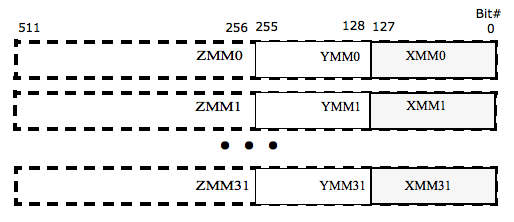
\includegraphics[width=\linewidth]{avx_mms.png}
    \caption{AVX512-Bit Wide Vectors and SIMD Register Set}
    \label{fig:avx_mms}
\end{figure}

AVX-512 not only takes advantage of using long vectors but also enables powerful high
vectorization features that can achieve significant speedup. Those features
include but not limit to:
\begin{enumerate}
  %\item using rich addressing mode which enables non-linear data access that can deal with non-contiguous data;
  \item providing a valuable set of horizontal reduction operations which applies to more types of reducible loop carried dependencies including both logical, integer and floating point of high speed math reductions;
  \item and permitting vectorization of loops with more complex loop carried dependencies and more complex control flow.
\end{enumerate}

\arm announced new Armv8 architecture embraced \sve - a vector extension for AArch64
execution mode for the A64 instruction set of the
Armv8 architecture~\cite{arm-v8-ref, ARMv8-Architecture}.
%arm-v8-sve,
Unlike other SIMD architectures, \sve does not define the size of
the vector registers, instead it provides a range of different values which permit vector
code to adapt automatically to the current vector length at runtime with the
feature of \emph{Vector Length Agnostic} (VLA) programming~\cite{Advanced-SIMD,vla-stencil}.
Vector length constrains in the range from a minimum of 128 bits up to
a maximum of 2048 bits in increments of 128 bits.

Message Passing Interface (\mpi)~\cite{mpi-forum} is a popular and efficient parallel
programming model for distributed memory systems widely used in scientific applications.
As many scientific applications operate on lagre amount of data, manipulating and opreating these data becomes complicated.
%
Especially for machine learning applications running on distributed systems,
processes need to use reduction operations for very large data sets to
synchronize updating the weights matrix.

Computation-oriented collective operations like MPI\_Reduce perform reductions on
data along with the communications performed by collectives.
These collectives normally require intensive CPU compute resources, which force
the computation to become the bottleneck and limit its performance.
However, with the presence of advanced architecture technologies introduced
with wide vector extension and specialized arithmetic operations, it calls for
MPI libraries to provide state-of-the-art design for advanced vector
extension (\sve and AVX-512~\cite{avx-info, Cebrian2019}) based versions.
We tackle the above challenges and provide designs and implementations
for reduction operations which are most commonly used by computation
intensive collectives - MPI\_Reduce, MPI\_Reduce\_local, MPI\_ALLreduce.
We propose extensions to multiple \mpi reduction methods to fully take
advantage of the AVX-512 capabilities such as vector product to efficiently
perform these operations.

This paper makes the following contributions:
%\begin{compactenum}
\begin{enumerate}
  \item analyzing AVX-512 hardware arithmetic instructions to speedup variety types of reduction operations and optimizing \mpi local reduction operations using related intrinsics which highly increased the performance;
  \item and performing experiments using our
      new reduction operations in the scope of \ompi on an local cluster comparising Intel processors.
      Experiment results demonstrate the efficiency
      of AVX-512 mathematical instructions and our implementation.
      Further more, provides useful insight and guideline on how vector
      ISA can be used in high performance computing platforms and softwares.
\end{enumerate}
%\end{compactenum}

The rest of this paper is organized as follows.
%Section~\ref{sec:motivation} motivates our study and provides use cases and
%background on the \sve instructions specific optimization in \mpi implementation in \ompi.
Section~\ref{sec:related} presents related researches taking advantage of AVX-512 and \sve for specific mathematics applications, together with a survey about optimizations of \mpi that taking advantages of novel hardwares.
Section~\ref{sec:design} describe the implementation details of our optimized reduction methods in the scope of \ompiusing AVX-512 intrinsics and instructions.
Section~\ref{sec:experiments} describes the performance difference between \ompi and AVX-512 optimized \ompi and provides a distinct insights on the how the new vector instructions can benefit \mpi.

\section{Related Work}\label{sec:related}
In this section, we survey related work on techniques taking advantages of
advanced hardwares or architectures.
%
Lim~\cite{Lim2018} explores matrix matrix multiplication based on blocked matrix multiplication
improves data reuse by data prefetching, loop unrolling, and the Intel AVX-512 to optimize the blocked matrix multiplications.
%
In another work~\cite{Kim19} presents the optimal implementations of single-precision and double-precision general matrix-matrix multiplication (GEMM) routines based on an auto-tuning approach with the Intel AVX-512 intrinsic functions.
%
Dosanjh et al.~\cite{tag-match} took the advantage of using AVX vector operation for
MPI message matching to accelerate matches which demonstrated the efficiency
of long vectors.
%
In another work~\cite{sve-stencil}, they leverage the characteristics of \sve to implement and optimize
stencil computations, ubiquitous in scientific computing which shows
that \sve enables easy deployment of optimizations like loop unrolling,
loop fusion, load trading or data reuse. However, all those work focus on using new instructions
for a specific application.
In our work we study AVX-512 enabled features in a more comprehensive way, and also provides
detailed analysis about the efficiency achievements of using related intrinsics.
We are focusing in networking runtime and not generic compute bound applications.

Additionally, different techniques and
efforts have been studied to optimize \mpi reduction operations. Jesper
~\cite{Neutral_MPI_Reduction} proposed a simple implementation of MPI library
internal functionality that enables MPI reduction operations to be performed
more efficiently with increasing sparsity of the input vectors. Also~\cite{gpu-reduce,Luo-adapt}
provided a design and implementation of computed-oriented collective using GPU accelerators.
Luo~\cite{Luo-adapt} offloaded the reduction operations to the GPU asynchronously by
using multiple CUDA streams which allowed the overlap of communications and reduction operations.
Michael~\cite{sparse-reduction} presented a pipeline algorithm for MPI Reduce
that used a Run Length Encoding scheme to improve the global reduction of sparse
floating-point data. Compared to those work, our \sve arithmetic reduction
optimization is more general at processor instruction level which  is more
straightforward and has no limitation of data representation and is using CPU resources only
without the need of external or extra hardwares.

\begin{figure}[h]
    \centering
    % trim={<left> <lower> <right> <upper>}
    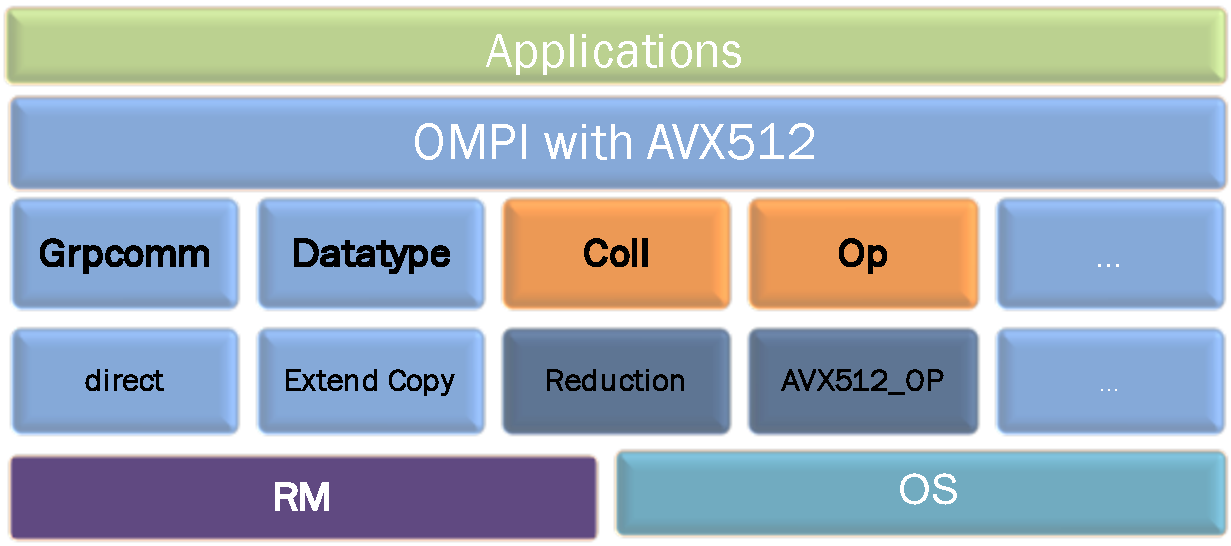
\includegraphics[width=\linewidth]{avx-mca.pdf}
    \caption{\ompi architecture. The orange boxes represent components with added AVX-512 reduction features. The dark blue colored boxes are new modules.}
    \label{fig:avx_mca}
\end{figure}

\begin{figure}[h]
    \centering
    % trim={<left> <lower> <right> <upper>}
    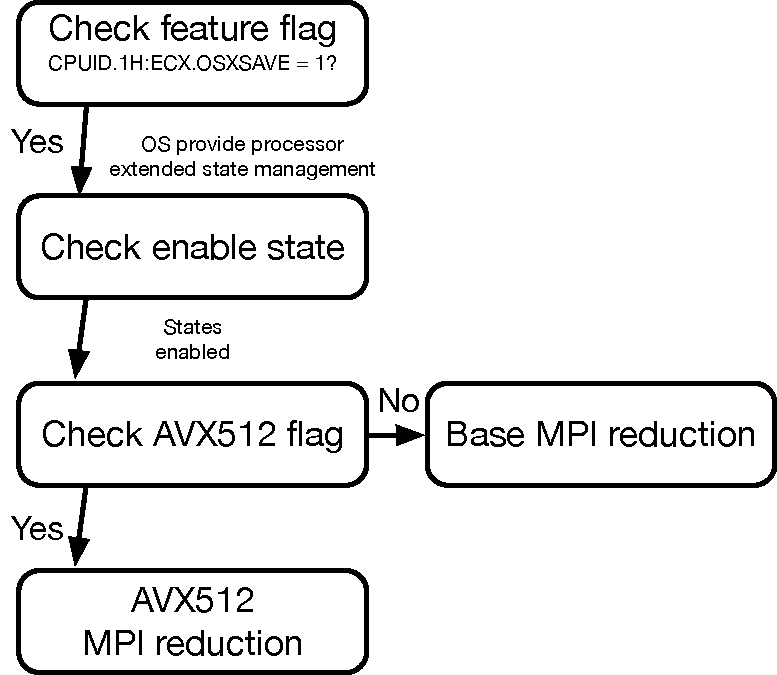
\includegraphics[scale=.45]{512-flow.pdf}
    \caption{Integrate and automatically activate the AVX component into the OMPI build system}
    \label{fig:512flow}
\end{figure}

\section{Design and implementation in OMPI}\label{sec:design}
We implemented AVX512 reduction operation work in a set of components in OMPI which is based on a Modular Component Architecture~\cite{dong_prrte} that permits easily extending or substituting the core subsystem with new features.
As shown below, we added our AVX512 optimization work in a components to OMPI architecture that implements all MPI reduction operations with AVX512 vector reduction instructions as in fig\ref{fig:avx_mca}; also we integrate our new module to automatically detect the hardware information to enable the AVX-512 reduction feature or fallback to the default basic module if it is not supported by the processor as show in fig\ref{fig:512flow}. To be noted, this component can be extend out the scope of local reduction to general mathematics and logic operations.

\begin{figure}[h]
    \centering
    % trim={<left> <lower> <right> <upper>}
    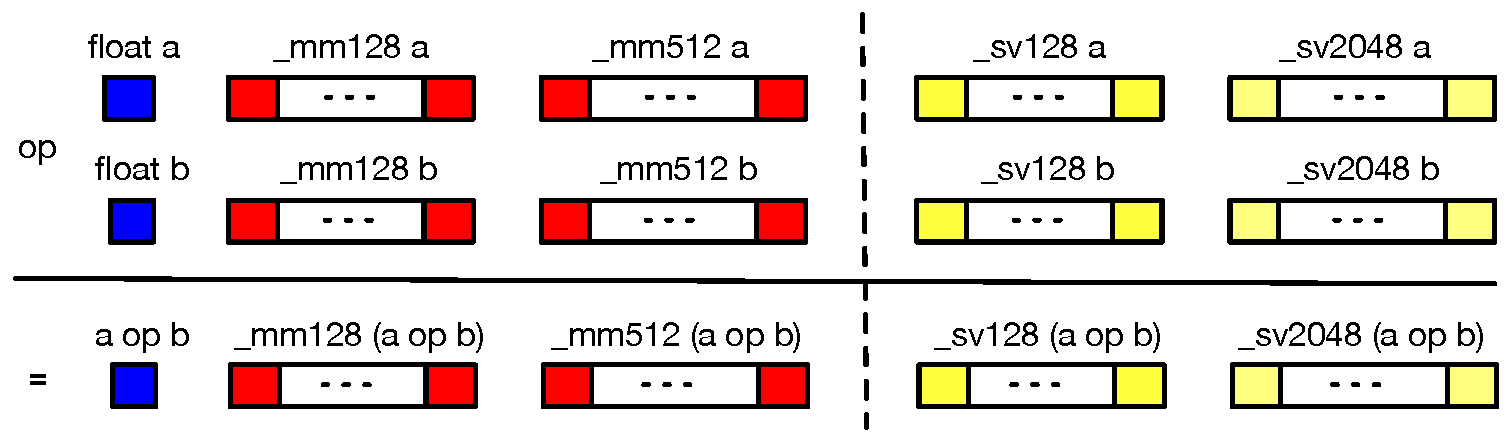
\includegraphics[width=\linewidth]{sse_avx.pdf}
    \caption{Example of single precision floating-point values using : (\colorbox{blue}{}) scalar standard C++ code, (\colorbox{green}{}) AVX SIMD vector of 4 values , (\colorbox{red}{}) AVX2 SIMD vector of 8 values, (\colorbox{yellow}{}) AVX512 SIMD vector of 16 values}
    \label{fig:sse_avx}
\end{figure}


A reduction is a common operation found in many scientific applications.
Those applications have large amounts of data level parallelism and should be able
to benefit from SIMD support for reduction operation.
Traditional reduction operation performs element by element of the input buffer
which executes as a sequential operation or it is possibly could be vectorized
under particular circumstance. Sometimes it may suffer from dependencies across
multiple loop iterations.
As show in Figure~\ref{fig:sse_avx} illustrates the difference between a scalar operation and
a vector operation for AVX, AVX2 or AVX512 respectively. An AVX512 SIMD-vector is able to store 8 double precision floating point numbers or 16 integer values, for example.
AVX-512 reduction instructions perform arithmetic horizontally across active elements of a
single source vector and deliver a scalar result. AVX-512 provides arithmetic
reduction operation for integer and float-pointing, also supports logical reduction
operations for integer type, an example format would be
\emph{\textit{\_\_m512i\ \_mm512\_add\_epi32\ (\_\_m512i a,\ \_\_m512i b)}}
this function produces the add results of two vectors.
This gives the chance to create AVX-512 intrinsic reduction in \mpi which
will highly increase the parallelization and performance of \mpi local reduction.
Also AVX-512 can performs scatter reduction operation with the accomplished
support of predicate vector register which behaves in a vectorized manner. This highly
expands the limitation of consecutive memory layout for reduction operation to non-contiguous
at the same time generic and efficient.

\begin{algorithm}[t]
\caption{AVX based reduction algorithm}\label{fig:reduce_algorithm}

\textbf{\textit{types\_per\_step}} \Comment{Number of elements in vector}\\
\textbf{\textit{left\_over}} \Comment{Number of elements waiting for reduction}\\
\textbf{\textit{count}} \Comment{Total number of elements for reduction operation}\\
\textbf{\textit{in\_buf}} \Comment{Input buffer for reduction operation}\\
\textbf{\textit{inout\_buf}} \Comment{Input and output buffer for reduction operation}\\

\begin{algorithmic}[1]
\Procedure{ReductionOp}{ $in\_buf, inout\_buf, count$ }
%\If {( $blocklen$ $\geqslant$ $svcntb$ )}
  \State $types\_per\_step$ = $vector\_length (512)$ / ($8$ $\times$ $sizeof\_type$)
%\EndIf
\For { $k \gets types\_per\_step $ to $ count$}
  \State {\_mm512\_loadu\_si512 from $in\_buf$}
  \State {\_mm512\_loadu\_si512 from $inout\_buf$}
  \State {\_mm512\_reduction\_op}
  \State {\_mm512\_storeu\_si512 to $inout\_buf$}
\EndFor
\If {( $left\_over$ $\neq$ $0$ )}
  \State Update $types\_per\_step >>= 1$
    \If {( $types\_per\_step$ $\leq$ $left\_over$)}
    \State {\_mm256\_loadu\_si256 from $in\_buf$}
    \State {\_mm256\_loadu\_si256 from $inout\_buf$}
    \State {\_mm256\_reduction\_op}
    \State {\_mm256\_storeu\_si256 to $inout\_buf$}
    \EndIf
\EndIf
\If {( $left\_over$ $\neq$ $0$ )}
  \State Update $types\_per\_step >>= 1$
    \If {( $types\_per\_step$ $\leq$ $left\_over$)}
    \State {\_mm\_llddqu\_si128 from $in\_buf$}
    \State {\_mm\_llddqu\_si128 from $inout\_buf$}
    \State {\_mm128\_reduction\_op}
    \State {\_mm\_storeu\_si128 to $inout\_buf$}
    \EndIf
\EndIf
\If {($left\_over$ $\neq$ $0$ )}
    \State {Duff device}
\EndIf
\EndProcedure
\end{algorithmic}
\end{algorithm}

%
For our optimized reduction opreation we use multiple methods try to achieve the most optimal performance as show in algorithm\ref{fig:reduce_algorithm}. For the main for-loop section we explicitly use AVX-512 bits vector loads and stores for memory operation instead of using memcpy. Because some systems and compilers may not provide the best assembling techniques of using ZMM registers to load and store. And the use vector mathematic operation to perform on those wide vectors.
%
Handling of the remainder we automatic use YMM registers processing elements that fit in the 256 bits registers.
For the last part of the remainder we use Duff's device which we manually implementing loop unrolling by interleaving two syntactic constructs of C: the do-while loop and a switch statement which helps the compiler to correctly optimize the device; it may also interfere with pipelining and branch prediction on some architecture. Table\ref{tab:parameters} shows
the variety of \mpifunc{Types} and \mpifunc{Ops} are supported in our optimiezed reduction operation module.
We can see our implenmentation supprts all combination of all types and operations in \mpi stardard.
Table\ref{tab:parameters1} lists the supported x86 instruction set architectures and related CPU flags from
legacy SSE to the latest AVX512 instruction sets.


\begin{table}
  \centering
  \caption{Supported types and operations}\label{fig:notations}
  \label{tab:parameters}
  \small
  \begin{tabular}{cclll}
    \toprule
    \texttt{\bf Types} & uint8 - uint64 & float & double \\
    \midrule
    \texttt{\bf MAX} & \checkmark & \checkmark & \checkmark \\
      \texttt{\bf MIN} & \checkmark & \checkmark & \checkmark \\
      \texttt{\bf SUM} & \checkmark & \checkmark & \checkmark \\
      \texttt{\bf PROD} & \checkmark & \checkmark & \checkmark \\
      \texttt{\bf BOR} & \checkmark & --- & --- \\
      \texttt{\bf BAND} & \checkmark & --- & --- \\
      \texttt{\bf BXOR} & \checkmark & --- & --- \\
      \bottomrule
  \end{tabular}
\end{table}

\begin{table}
  \centering
  \caption{Supported CPU flags}\label{fig:cpuflags}
  \label{tab:parameters1}
  \small
  \begin{tabular}{cclll}
    \toprule
    \texttt{\bf Instruction Sets} &     &    CPU flags     &  \\
    \midrule
    \texttt{\bf AVX} & AVX512BW & AVX512F & AVX2 & AVX \\
      \texttt{\bf SSE} & SSE4 & SSE3 & SSE2 & SSE \\
      \bottomrule
  \end{tabular}
\end{table}

\section{Performance tool evaluation}\label{sec:perf}
In the section, we study the benefits of our AVX-512 intrinsics enabled \ompi by using PAPI~\cite{papi} -- tool that can measure application performance in these increasingly complex environments must also increase the richness of their measurements to provide insights into the increasingly intricate ways in which software and hardware interact.
PAPI (the Performance API) has provided consistent platform and operating system independent access to CPU hardware performance counters.

Figure~\ref{fig:papi_ins} and figure~\ref{fig:papi_br} illustrate the instruction count details
of branching instructions and load/store instructions of both AVX512 implementation and the default
element-wise reduction method. By using long vectors we largely decreased the "for loop" of the reduction
operaion. Consequently, the AVX512 code has much less control and branching instructions. For the load and store
instruction, longer vector can load and store more elements for each instruction compared to non-vector load and store, which means that we neeed less load and store instrutions dealing with the same amount of reduction data.


%PAPI_BR_UCN  0x8000002a  Yes  Unconditional branch instructions
%PAPI_BR_CN   0x8000002b  No   Conditional branch instructions
%PAPI_BR_TKN  0x8000002c  Yes  Conditional branch instructions taken
%PAPI_BR_NTK  0x8000002d  No   Conditional branch instructions not taken
%PAPI_BR_MSP  0x8000002e  No   Conditional branch instructions mispredicted
%PAPI_BR_PRC  0x8000002f  Yes  Conditional branch instructions correctly predicted
%PAPI_BR_INS  0x80000037  No   Branch instructions
%PAPI_TOT_INS 0x80000032  No   Instructions completed
%PAPI_LD_INS  0x80000035  No   Load instructions
%PAPI_SR_INS  0x80000036  No   Store instructions
%PAPI_LST_INS 0x8000003c  Yes  Load/store instructions completed


\begin{figure}[h]
    \centering
    % trim={<left> <lower> <right> <upper>}
    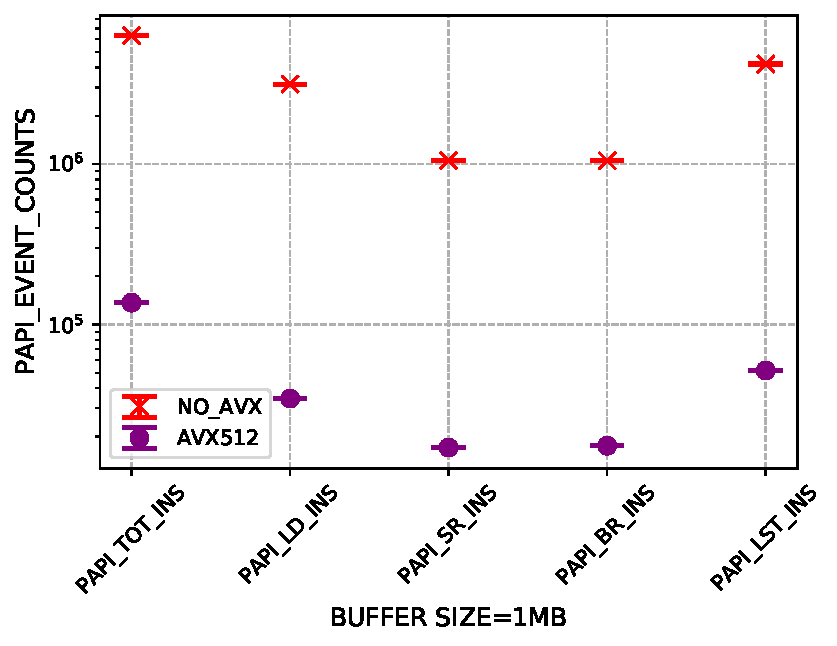
\includegraphics[width=\linewidth]{papi_ins.pdf}
    \caption{MPI\_SUM with AVX-512 enable and disable with PAPI instruction events overview}
    \label{fig:papi_ins}
\end{figure}

\begin{figure}[h]
    \centering
    % trim={<left> <lower> <right> <upper>}
    \includegraphics[width=\linewidth]{papi_br.pdf}
    \caption{MPI\_SUM with AVX-512 enable and disable for PAPI branch instructions}
    \label{fig:papi_br}
\end{figure}


\section{Experimental evaluation}\label{sec:experiments}
Experimented on a local cluster which is a Intel(R) Xeon(R) Gold 6254 based server running at 3.10 GHz. Our work is based upon OMPI master branch, revision \#75a539. Each experiment is repeated 30 times and we present the average. For all experiment we use a single node with one process, because our optimization aims to improve the performance of local reduction operation.

This section compares the performance of reduction operation with two
implementations.
For \ompi default operation base module it
performs element wise reduction operation across two input buffers. For each loop iteration
it processes two elements. Our new implementation we use AVX-512 vector reduction instruction
executing reduction operation on the same inputs but for each iteration it
deals with two vectors containing all the elements within the vectors which represents
a vector-wise operation.
For the reduction benchmark we use the \mpifunc{Reduce_local} function call to
perform the local reduction for all supported MPI operations using an array with different sizes.

We present to compare arithmetic SUM and logical BAND.
For the experiments we flushed cache to ensure we are not reusing cache for fair comparison.

Figure~\ref{fig:avx_sum} and figure~\ref{fig:avx_band} show the result for the
\mpifunc{SUM} and \mpifunc{BAND}, due to the limited length of the paper, we cannot
include the assemble code here. But it should be noted that the compiler, despite
the optimization flags provided, did not generate auto-vectorized code for the
default \ompi. Our optimization using intrinsics which gives us completely control of the low
level details at the expense of productivity and portability.

Results demonstrate that with AVX512-enabled operation it is 10X faster than element-wise operation. We also compare MPI operation together with memcpy which indicates the peak memory bandwidth. For mpi reduction operation it needs 2 loads, 1 store and additional computation. For memcpy it only needs 1 load and 1 store.
The result shows even with computation included AVX512 reduction operation achieves a similar level of memory bandwidth as memcpy.

\begin{figure}[h]
    \centering
    % trim={<left> <lower> <right> <upper>}
    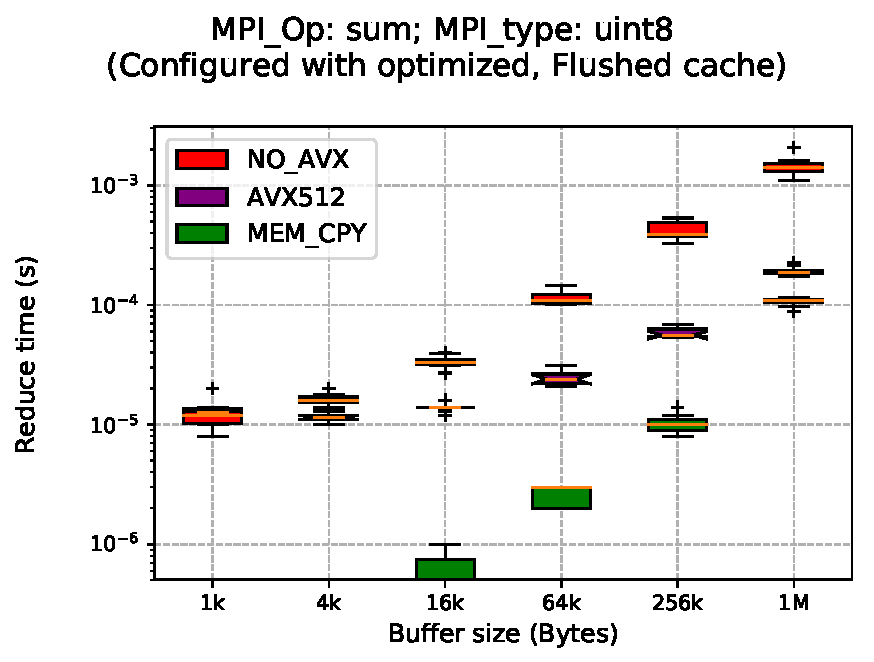
\includegraphics[trim={0 0 0 1.5cm},clip, width=\linewidth]{avx_sum.pdf}
    \caption{Comparison of MPI\_SUM with AVX-512 reduction enable and disable for MPI\_SUM together with memcpy}
    \label{fig:avx_sum}
\end{figure}

\begin{figure}[h]
    \centering
    % trim={<left> <lower> <right> <upper>}
    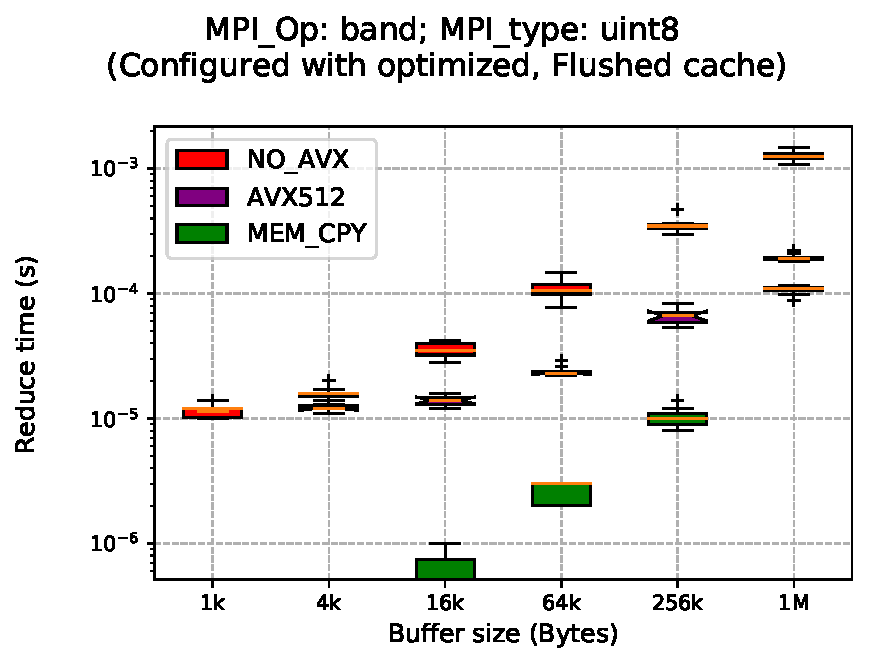
\includegraphics[trim={0 0 0 1.5cm},clip,width=\linewidth]{avx_band.pdf}
    \caption{Comparison of MPI\_BAND with AVX-512 reduction enable and disable for MPI\_SUM together with memcpy}
    \label{fig:avx_band}
\end{figure}

\section{Communication Models Coverage and Application Evaluation}\label{sec:application}
Over the past few years, advances in deep learning have driven tremendous progress in image
processing, speech recognition, and forecasting. Currently, one of the significant challenges
of deep learning is it is a very time-consuming process. Designing a deep learning model
requires design space exploration of a large number of hyper-parameters and processing big data.
Thus, accelerating the training process is critical for our research and development.
Distributed deep learning is one of the essential technologies in reducing training time.
In this section we investigate an application Horovod~\cite{sergeev2018horovod} - an open-source component of Michelangelo's deep learning toolkit which makes it easier to start and speed
up distributed deep learning projects with TensorFlow.

The important aspect to understand is that in deep learning it needs to calculate and update the gradient
in order to be able to adjust the weights. Without this learning can't happen. In order to calculate that gradient, it needs to process all of the data which is normally very large. When such data is too big it needs to parallelize these calculations. This means that it will have distribted computing nodes working in parallel on a subset of the data. When each of these processing units or workers (they could be CPUs, GPUs, TPUs, etc.) is done calculating the gradient for its subset, they then need to communicate its results to the rest of the processes involved. Actually, every process/node needs to communicate its results with every other process/node.

Horovod utilize Open MPI to launch all copies of the TensorFlow program. MPI then transparently sets up the distributed infrastructure necessary for workers to communicate with each other. All the user needs to do is
modify their program to average gradients using an Allreduce operation. Conceptually Allreduce has every process share its data with all other processes and applies a reduction operation. This operation can be any reduction operation, such as sum, multiplication, max or min. In other words, it reduces the target arrays in all processes
to a single array and returns the resultant array to all processes. Horovod uses a ring-allreduce approach as an optimal method in the sense of both usability and performance.
Ring-allreduce utilizes the network in an optimal way if the tensors are large enough, but does not
work as efficiently or quickly if they are very small. Horovod introduced Tensor Fusion - an algorithm that fuses tensors together before it calls ring-allreduce. The fusion method allocates a largde fusion buffer and execute the allreduce operation on the fusion buffer.
In the ring-allreduce algorithm, each of N nodes communicates with two of its
peers $2 * ($N - 1$)$ times. During this communication, a node sends and receives chunks of the data
buffer. In the first $N - 1$ iterations, received values are added to the values in the node's buffer. In
the second $N - 1$ iterations, when each process receives the data from the previous process it'd then
apply the reduce operator, and then proceeds to send it again to the next process in the ring which is bandwidth optimal~\cite{allreduce-optimal}. We can see that during the allreduce processing phase, $P * ($N - 1$)$ reduction operations occured with big fusion buffer size. Consequently, our AVX512 enabled reduction operations can particularly improve the performance of the collective operation.

We conducted our experiments on Stampede2 with Intel Xeon Platinum 8160 ("Skylake") nodes, each node has 48 cores.
We experimented with TensorFlow CNN benchmarks using Horovod with tensorflow-1.13.1.

\begin{figure}[h]
    \centering
    % trim={<left> <lower> <right> <upper>}
    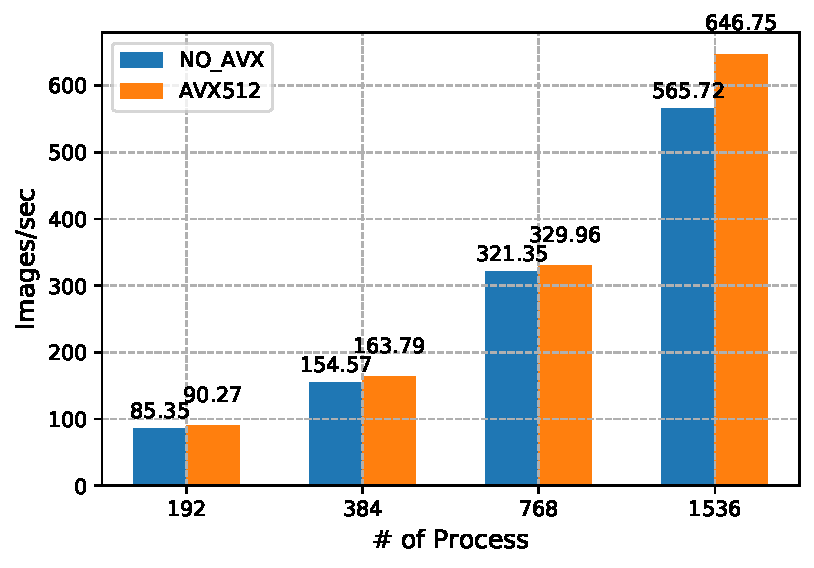
\includegraphics[width=\linewidth]{horovod_tacc.pdf}
    \caption{tf\_cnn\_benchmarks results using distributed Horovod (model: alexnet) on stampede2 with AVX512 enabale and disable}
    \label{fig:horovod_tacc}
\end{figure}

Figure~\ref{fig:horovod_tacc} shows the performance comparison of tf\_cnn\_benchmarks~\cite{cnn_Tensorflow} trained with Horovod
using alexnet model with our AVX512 enabled reduction operation and the default reduction operation in \ompi.

Nowadays, more and more systems in HPC feature a hierarchical hardware design: Shared memory nodes
with several multi-core CPUs are connected via a network infrastructure. This trend has disrupted the long status-quo in which parallel applications are written in \mpi, and has promoted the emergence of multiple alternatives for programming parallel systems.

On one hand, one may encounter programming styles that combines distributed memory parallelization between nodes separated by the interconnect, and shared memory parallelization, or GPU acceleration inside each node. On the other hand, parallel applications may alternate between
library calls that utilize different programming environments and programming models
to perform internode communication, for example, message passing and parallel global address space models may coexist in the same application. Consequently,
runtime environment needs to handle the cooperations between different programming models. Together,
failure detection and management techniques need to be expanded across different models.

In this section we investigate application support of \ourwork with different programming models.
Our interests focus on 1) demonstrating how our generic capabilities can support multiple programming languages, 2) how much overhead (if any) is incurred on both two-sided (e.g., \mpi) and one-sized programming models (e.g., \oshmem), and 3) provide the blueprints for supporting applications using multiple programming models.
In hybrid applications and models, there is no ``standard'' method by which programming models can coordinate.
For example, \mpi has the standard \mpifunc{Init} function that must be called to initialize the
library – providing a "hook" within that function to notify others that it has been called.
In contrast, OpenMP does not have an explicit call to "init" and is instead initialized on first use; older versions of \oshmem also allow implicit initialization.
Figure~\ref{fig:prrte.with.oshmem} shows how to coordinate between two different models. We can see
that as both communication libraries employ the PMIx library to interface with the runtime and job scheduling system,
the different programming languages have a common interface to exchange information.
The calls into PMIx\_Init from each programming model enters the same code space and offers an opportunity for coordination.
The event notification mechanism within PMIx can then be used to share the information and coordinate between those models.

To evaluate the overhead on performance from \ourwork
in \mpi and \oshmem applications, we use the heavily communication-bound benchmark Graph500~\cite{graph500}.
Graph500 is an open specification effort to offer a standardized graph-based
benchmark across large-scale distributed
platforms which captures the behavior of common communication-bound graph algorithms.
Graph500 differs from other large-scale
benchmarksm such as HPL, and HGPGMG in the way it primarily highlights data access patterns.
Graph500 performs a breadth-first search (BFS) in
parallel on a large randomly generated undirected graph. Our experiments use a
the open source project \oshmem Benchmark (OSB) suite~\cite{g500shmem} that features both \mpi and \oshmem based
Graph500 implementations. For the application setting we use \texttt{\bf $scale\_factor = 20$, $edge\_factor = 16$ }
which generates an undirected graph with \texttt{\bf $2^{scale\_factor}$} vertices and
\texttt{\bf $2^{scale\_factor}*edge\_factor$} edges. The benchmark collects the statistics
of the generation of the breadth-first search tree of 64 randomly selected vertices. It also
collect the statistics of validation time which ensures that all connected components are visited
which generate large amount of communications. For the experiments, we use NERSC Cori with 1K nodes. This results in a deployment with 32K \mpi  ranks, or 32K \oshmem Processing Elements (PEs).

\section{Conclusion}\label{sec:conclusion}
In this paper, we demonstrated the benefits of Intel AVX512f and AVX2 vector operations. We
addressed the performance advantages of different features introduced by AVX
with longer vector length compared to non-AVX implementations. Furthermore,
we extended the implementation of our investigation and analysis to introduced
an optimistic \mpi optimization.
%
We introduced
a new reduction operation module in \ompi using AVX512 intrinsics supporting
different kinds of \mpi reduce operations for multiple \mpi types. We
demonstrated the efficiency of our vector reduction operation by a benchmark
calling \mpifunc{Local_reduce}. From $VL=128$ to $VL=2048$ bits we decreased the
instruction count from 50\% to $30 \times$. To further validate the performance improvements,
experiments are conducted using Fujitsu's A64FX processor. For \mpifunc{Local_reduce} with $VL=512$
SVE based reduction operation is $4 \times$ faster.
Our analysis and implementation of
\ompi optimization provides useful insights and guidelines on how \arm \sve
vector ISA can be used in actual high performance computing platforms and
software to improve the efficiency of parallel runtimes and applications.

\section*{Acknowledgement}
%
This material is based upon work supported by the National Science Foundation under Grant No. (1725692); and the Exascale Computing Project (17-SC-20-SC), a collaborative effort of the
U.S. Department of Energy Office of Science and the National Nuclear Security Administration.

%\balance
%
%
\bibliographystyle{ACM-Reference-Format}
\bibliography{sample-base}

\end{document}

%%
%% End of file `sample-sigconf.tex'.
